\documentclass[]{article}
\usepackage[english]{babel}
\usepackage{amsmath}
\usepackage{graphicx}
\usepackage[hypcap=false]{caption}
\usepackage{subcaption}
\graphicspath{ {./images/} }
\usepackage{hyperref}
\hypersetup{
	hidelinks
	}

\title{Artificial Intelligence in Cybersecurity: Assignment 3}
\author{Brandon Hosley}
\date{\today}

\begin{document}
	\maketitle
	
\section{Introduction}

In this article \cite{Jeon2021} Jeon et al. develop a framework that is intended to 


\section{Data Sources}

% Describe the data used in this paper including source, sample, attribute, etc. (10 points)


\section{Algorithm}



% Draw a flowchart of the algorithm for visualization (10 points)
\begin{figure}[h]
	\centering
	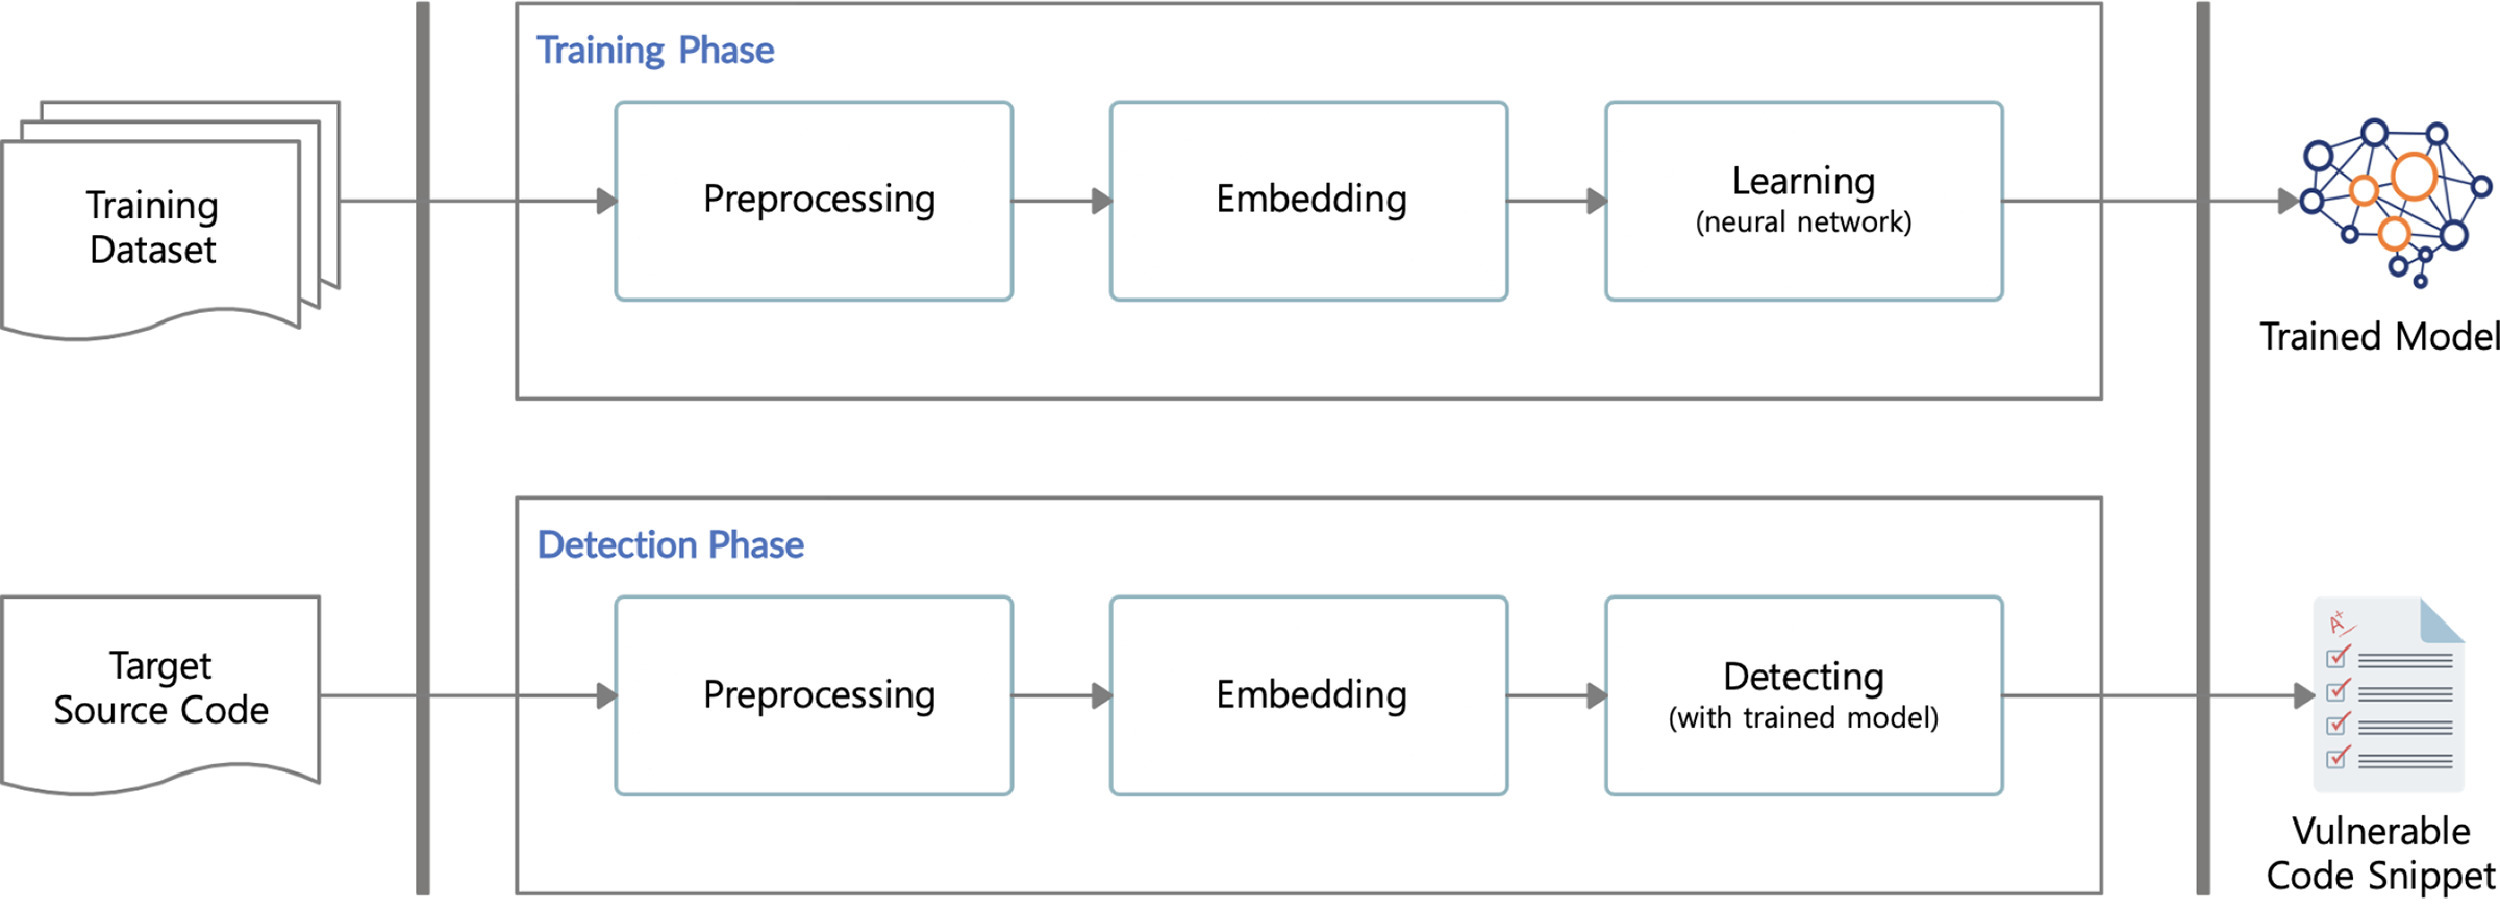
\includegraphics[width=\textwidth]{Algorithm}
	\caption{Deep4SNet \cite{Jeon2021}}
\end{figure}


\section{Results}

% Explain the experimental results in detail from your understanding (10 points)


\section{Advantages and Disadvantages}

% Discuss the advantages from your understanding (10 points)
The primary advantage and overall goal of this framework is to automatically check code for known vulnerabilities. 
AutoVAS does this with good results.
By doing so automatically users will be better equipped to evaluate software on an ongoing basis.
AutoVAS can continually be updated with new sample sets and used to evaluate a code-base, all without a significant introduction of overhead to the testers.
The method of execution (static evaluation) is safer on the training side, and can be accomplished faster.
Additionally, the results from the neural network method tends to perform better at identifying vulnerabilities that are functionally similar to known vulnerabilities rather than linguistically similar in contrast to other popular methods.
The methods that the team compared are code similarity and pattern recognition frameworks. 
AutoVAS should also outperform these types of methods especially against novel exploits or novel implementations of known exploits.
All of this allows vulnerability analysis to meet the speed of Automatic Exploit Generation (AEG).

% Discuss the disadvantages from your understanding (15 points)
The framework is not without disadvantages and the research team was very candid about these shortcomings.
The framework is very language dependent in this implementation.
At this time it only functions on C//C++ source code.
Beyond the language barrier this also presents a problem by the need for access to the source-code.
While this may be feasible for software developers testing in-house, it will not work for third party testers, whether they are testing as a service or testing software they wish to use as a consumer.
The team pushes the speed benefits of source code analysis, but a more generalized approach might make the framework more applicable to real world application.

\section{Improvements}

% Provide the specific ideas to improve the algorithm. General ideas are not allowed. (15 points)
As with the discussion of disadvantages of OpenVAS the development team was very candid regarding areas for improvement.
Two major areas of improvement would make the framework far more usable in two slightly different arenas.

The first is for the framework to be adapted to be language agnostic or especially to work on binaries.
By becoming language agnostic this framework can be better adapted to larger code-bases, many of which span multiple programming languages. 
This may just mean agnosticism in the source code, but more possibly this may approach binaries or executable code as well.
If done in this manner it would expand the usability of the framework to test software by entities without the source code; third party testers or consumers themselves.

Next is to output more than just a binary determination to more specifically describe the reasoning for the vulnerable determination.
The team suggested that this may be accomplished using Interpretable Machine Learning, which allows outputs to be more easily interpreted.
This may describe the type of vulnerability observed which will better equip developers with direction to remedy the issue.
Additionally, this may inform a consumer about the potential risk of using the software which may be a risk acceptable for their situation.
Even more useful, but likely more difficult would be an output of the location of the defect origin.
This would greatly assist the developers in their remediation efforts by directing them immediately to the concerning items.
Even if the nature of the vulnerability is not described the developers would be far better equipped to make that determination just with the location description.


\clearpage
\bibliographystyle{acm}
\bibliography{\jobname}
\end{document}